\chapter{Non parametric estimation of the probability density function(???)}

We can estimate the probability density function in a non parametric way as follows:
\begin{equation}
    \begin{aligned}
        \hat{f}_N(x) &= \frac{\hat{F}_N(x+\frac{h}{2}) - \hat{F}_N(x-\frac{h}{2})  }{h}\\
        \hat{f}_N(x) &= \frac{\#\{x_k\::\: x - \frac{h}{2}\le x_k \le x + \frac{h}{2}\}}{Nh}

        
    \end{aligned}
\end{equation}

\nt{The above is essentially 1 bin of a histogram, non parametric estimation just means creating a histogram with smaller and smaller bins}
\dfn{Kernel function}
{
    An example of a kernel function (Parzen kernel(???)) would be:
    \begin{equation}
        K(v) = \begin{cases}
            1 \text{ as } \norm{v} \le \frac{1}{2}\\
            0 \text{ otherwise}
        \end{cases}
    \end{equation}
    %% plot


\begin{center}
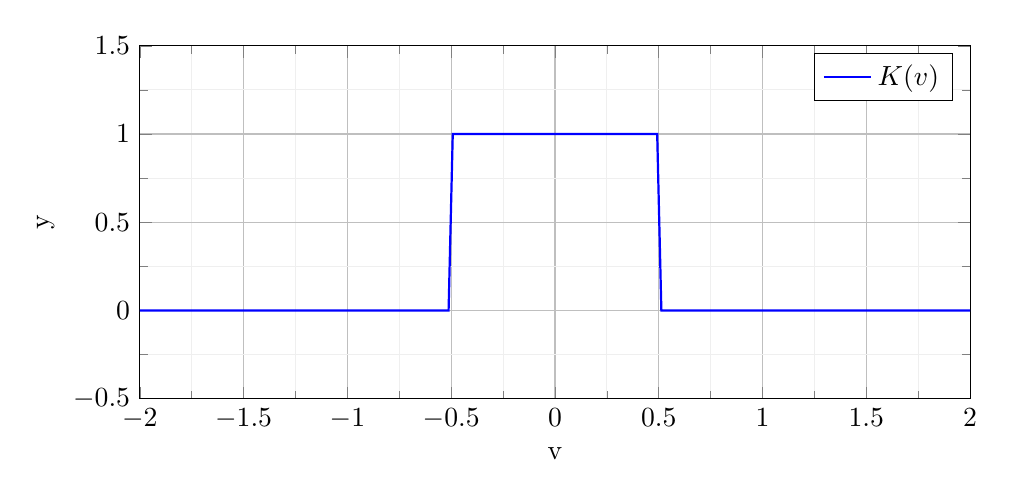
\begin{tikzpicture}
 
\begin{axis}[
    xmin = -2, xmax = 2,
    ymin = -0.5, ymax = 1.5,
    grid = both,
    minor tick num = 1,
    major grid style = {lightgray},
    minor grid style = {lightgray!25},
    width = \textwidth,
    height = 0.5\textwidth,
    xlabel = v,
    ylabel = y]
    \addplot[
        domain = -2:2,
        samples = 200,
        thick,
        blue,
        ] 
        {
        (x > -0.5)*(1)*(x < 0.5)*(1) + 0
        };

    \legend{$K(v)$
           }
\end{axis}
 
\end{tikzpicture}
\end{center}

    When is $K(\frac{x_k-x}{h}) = 1$? This example shows that $K(v)$ plays the role of a selector function, as it will be 1 only when $\norm{x_k-x} \le \frac{1}{2}h$
    \\
    By an appropriate choice of h we can use K(v) to approximate the probability density function.
}

\thm{Kernel probability estimation}
{
    \begin{equation}
        \hat{f}_N(x) = \frac{1}{Nh}\Sigma_{k=1}^{N}K(\frac{x_k-x}{h})
    \end{equation}

    Limit properties ($N \rightarrow \infty$):\\
    How to set $h$ asymptotically?
    \begin{equation}
        \text{If } N \rightarrow \infty
        \begin{cases}
            h(N) \rightarrow 0 \text{ then bias } \hat{f}_n(x) \rightarrow 0\\
            Nh(N) \rightarrow \infty \text{ then } \text{var}\hat{f}(x) \rightarrow 0
        \end{cases}
    \end{equation}

    This means that $h(N) \in \mathcal{o}(\frac{1}{N})$ FIX THIS <<<<<, e.g. it has to increase no faster than $\frac{1}{B}$, so for example $h(N) = \frac{1}{\sqrt{N}}$

    \nt{
    In the multidimensional case we get a more restrictive condition on asymptotic behaviour:

 \begin{equation}
        \text{If } N \rightarrow \infty
        \begin{cases}
            h(N) \rightarrow 0 \text{ then bias } \hat{f}_n(x) \rightarrow 0\\
            Nh(N)^{2} \rightarrow \infty \text{ then } \text{var}\hat{f}(x) \rightarrow 0
        \end{cases}
    \end{equation}
Which means that $h(N)$ tends to 0 much more slowly than in the 1D case
    }
}




\ex{Learning of recognition}
{
    Let's say we have 2 classes and 1 feature about them, e.g. the class of men and women, and the feature of their height, so d = 1.



\begin{center}
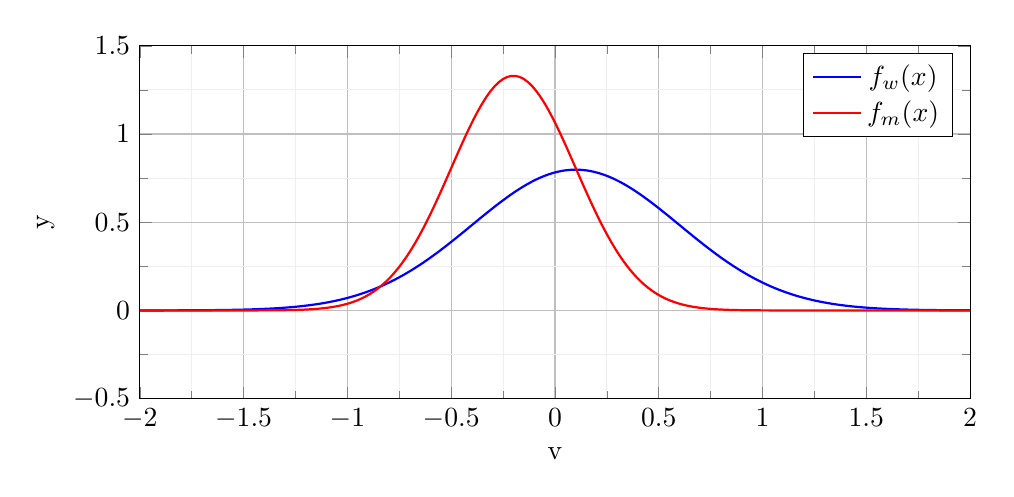
\begin{tikzpicture}
 
\begin{axis}[
    xmin = -2, xmax = 2,
    ymin = -0.5, ymax = 1.5,
    grid = both,
    minor tick num = 1,
    major grid style = {lightgray},
    minor grid style = {lightgray!25},
    width = \textwidth,
    height = 0.5\textwidth,
    xlabel = v,
    ylabel = y]
    \addplot[
        domain = -2:2,
        samples = 200,
        thick,
        blue,
        ] 
        {
            exp(-0.5*((x-0.1)/0.5)^2)/(0.5*sqrt(2*3.1415)) 
        };

    \addplot[
        domain = -2:2,
        samples = 200,
        thick,
        red,
        ] 
        {
            exp(-0.5*((x+0.2)/0.3)^2)/(0.3*sqrt(2*3.1415)) 
        };




    \legend{$f_w(x)$,
            $f_m(x)$
           }
\end{axis}
\end{tikzpicture}
\end{center}

%%ADD a plot for intersection
Recognition algorithm:
\begin{equation}
    \begin{cases}
        x > D \rightarrow  \text{Decision = Man}\\
        x < D \rightarrow  \text{Decision = Woman}\\
    \end{cases}
\end{equation}
\nt{If the costs of error2 and error1 are different} D can change\\
If $\#?????$


}






